\chapter{Literature Review}
\label{cha:LitReview}

\section{Why Map the Internet?}
\label{sec:LitReviewWhyMap}

The main aim of this project is to embed a representation of the internet into hyperbolic space and produce a visualisation of this embedding. In order to fully understand why this is useful, we must ask the question: Why do we need a map of the internet? 

Understanding the physical structure of the internet is something that network engineers have to deal with every day, however it can often be difficult to pinpoint problems in networks. For example, in standard Ethernet networks, the presence of a loop can often create a broadcast storm which can render entire parts of a network unusable due to packet flooding. If an accurate map of the network is known in advance then it is possible for an engineer to locate the fault more quickly as they can compare this map to the current state of the network and check to see if any new connections have been added which may be causing the loop. 

While maps may assist engineers on small scale problems they can also assist in diagnosing problems which affect the internet on a more global scale. For example, despite the extreme interconnectedness of the internet it is still possible for a specific node or link to become congested. Congestion of a node or link can cause severe packet loss making data transmission unreliable across the affected area. Having an accurate map of the internet would allow for quick diagnosis of the fault, as well as pinpointing the cause. Though it may have been possible without a map to easily find the affected nodes or links it would be far more difficult to find the cause of the issue. With a map, it is possible to identify features such as a large number of new nodes which may have caused increased data transmission across the affected area. Additionally, a map of the internet with a geographical element may assist in locating pairs of nodes which could receive additional links or additional bandwidth on existing links.

\section{The World Wide Web}

\label{sec:LitReviewWWW}
Munzner et al undertook previous work which consisted of visualising the structure of the World Wide Web (WWW) in hyperbolic space \cite{munzner_visualizing_1995}. Though this may seem similar to the aim of this project there are key differences between the internet and the WWW which distinguish this project. In order to appreciate these differences it is necessary to understand what the WWW is. 

While the internet is a physical concept, the WWW is not. The WWW represents the data that users of the internet can view, specifically it contains text data formatted using the Hypertext Mark-up Language (HTML) standard which allows users to view as well as navigate this data. This is done using a type of application known as a \textit{web browser}. Web browsers allow users to navigate to web addresses (\textit{www.google.co.uk} for example) and view information stored at these addresses. The user views web pages which can also contain links to other web pages, users can follow these links in their browser to visit these other pages. 

If we imagine each web page as a node in a graph and the links between pages as edges then it possible to construct a graph which represents the WWW or a subset thereof. Recall, however that the internet is, at a basic level, a graph too. While these two graphs have similarities they are fundamentally different. While the graph that represents the internet contains at most a single node per physical device, it is possible for the graph that represents the WWW to contain multiple nodes per physical device. This is explained by having a node in the internet graph which hosts multiple pages in the WWW, which is extremely common. Due to this one to many mapping between physical internet nodes and WWW nodes the graphs of the internet and WWW are very different. 

A further difference between the two concepts is that links in the WWW have a direction whereas internet links do not. It would be necessary for any graph representing the WWW to be able to represent directional links between nodes.  The internet graph does not need such complexity and can be represented with only bi-directional links. 

\section{Autonomous Systems}
\label{sec:LitReviewAutSystems}

Though this project aims to map the internet, there are many different ways in which this can be done and it must be done in a way that is possible with the available resources. It is not sufficient to simply state that this project will create a map of the entire internet as it is not possible to obtain the correct data to do this. Instead a representation of the internet which is useful and for which sufficient data exists must be chosen on which to base the mapping.

\textit{Autonomous systems} are an ideal candidate for this as the data is readily available \cite{introduction_ripe_api}. However this only satisfies half of the requirements; are autonomous systems useful as a representation of the internet?

An autonomous system (AS) is "a portion of the internet under a single administrative authority" of which there are more than 10,000 \cite{di_battista_computing_2003}. It is these ASes which provide long distance routing over the internet while effectively abstracting their internal routing away from the perspective of those outside of the system. Routing information is exchanged between ASes using the Border Gateway Protocol (BGP) \cite{secure_ieee}. Due to this abstraction of internal routing it is both difficult and unnecessary to visualise the internals of an AS, indeed many administrators of ASes wish to keep their internal routing protocols secret for security reasons. Regardless of how an AS operates internally it is only possible to visualise its contribution to the internet as a whole externally. 

Further, the structure of combined ASes creates a natural tree structure. This is evident when the different types of AS are examined. In order to provide routing capabilities across the internet it is necessary for ASes to provide routes to forward traffic to other ASes. This type of AS, the \textit{provider} type, constitutes an internal node in this tree structure. Provider ASes would typically belong to internet service providers (ISPs). Leaf nodes represent any AS which does not provide routes to any other AS, for example an AS owned by a university. This type of AS will be referred to as a \textit{consumer} AS.

Though this representation may seem sound, there are issues which prevent the internet from being represented as a true tree. It is possible for a consumer AS to link physically to several provider ASes while not advertising routes to these provider ASes. This consumer AS would effectively have two parent nodes but appear as a leaf node with a single parent from the perspective of the parents. This configuration is extremely common as often organisations wish to have multiple connections to the internet through different providers in case a single connection fails. This type of AS is known as "multihomed" \cite{calvert_modeling_1997}.

Further, the graph of AS connections is not a true tree due to the links between provider ASes effectively being undirected \cite{di_battista_computing_2003}. A tree must have directional links in order to determine which nodes are parents and which are children. This distinction becomes blurred when using a tree to describe the structure of the internet as all provider ASes are effectively equal, it is not possible to say that one provider AS is the child of another and this assertion has no meaning. A further, but minor, difference is that such a tree has no root node. 

These issues make it impossible to represent the internet, at the level of autonomous systems, as a tree but it could be said that the structure is \textit{tree-like} with internal and leaf nodes which provide a hierarchical structure which can be represented as a graph. TODO!!!

\section{Hyperbolic Space}
\label{sec:LitReviewHyperbolicSpace}

Hyperbolic space (or, more broadly, hyperbolic geometry) is by no means a recent concept and was postulated by Carl Friedrich Gauss in 1824 \cite{ratcliffe_foundations_2006}. In order to understand what hyperbolic geometry is, it is first necessary to review what is often described as standard: Euclidean geometry.

Euclidean geometry (postulated by Euclid in around 300 B.C. \cite{ratcliffe_foundations_2006}) is based upon five postulates, which Euclid described as follows \cite{ratcliffe_foundations_2006}:
\begin{enumerate}
\item \textit{A straight line may be drawn from any point to any other point.}
\item \textit{A finite straight line may be extended continuously in a straight line.}
\item \textit{A circle may be drawn with any centre and any radius.}
\item \textit{All right angles are equal.}
\item \textit{If a straight line falling on two straight lines makes the interior angles on the same side less than two right angles, the two straight lines, if extended infinitely, meet on the side on which the angles are less than two right angles.}
\end{enumerate}

The first four of these postulates seem both simple and natural, however the fifth is more involved and it is not immediately apparent what is being described by it. Euclid's fifth postulate effectively states that given a straight line and a point, there is only \textbf{one} straight line which passes through the point and is parallel to the original straight line. 

When considering the first four postulates it is easy to see that they should simply be accepted without proof due to their simplicity. However, the fifth postulate cannot be so easily accepted. A solution to this is to attempt to prove the fifth postulate using the others, something which was attempted for over two thousand years \cite{ratcliffe_foundations_2006} but was not possible. The only remaining hypothesis is that the fifth postulate is not required for a definition of a geometry.

This seems absurd, as it is relatively simple to demonstrate in two dimensional Euclidean geometry that the fifth postulate holds, using only a piece of paper and a pencil. However, this does not prove that the postulate holds in all cases, only in this one instance. In order to refute the postulate, it is necessary cast out this rigid view of a flat plane and to consider other geometries in which to work. 

If, instead of a plane, all geometry took place on the surface of a sphere then very different behaviour is observed. Of course, the surface of the sphere is a two dimensional space but with one key difference: it is finite. On this finite space a straight line is any which is a great circle of the sphere. In this case, it is clear that any straight line must have \textbf{zero} straight lines which are parallel to it, as all pairs of great circles must meet at exactly two points. This is in direct violation of Euclid's fifth postulate, however this \textit{spherical geometry} still constitutes a valid definition of geometry. Clearly, the fifth postulate is not required in order to define a geometry.

This being the case would suggest that geometries can be defined in such a way that a straight line has any number of parallels through a point. Indeed, a geometry exists in which each straight line has many parallels through a point: \textit{hyperbolic geometry} \cite{munzner_visualizing_1995}. This type of geometry is more difficult to visualise in Euclidean space than spherical geometry but is not restricted to a finite plane. Unlike spherical geometry, which has a \textit{constant positive curvature}, hyperbolic geometry has a \textit{constant negative curvature} which, put simply, causes the amount of available space to expand in every direction. This statement becomes more evident when the area of a circle in each geometry is considered. In euclidean space, a circles area grows linearly with its radius whereas in hyperbolic space this growth is exponential \cite{munzner_visualizing_1995}.

Another interesting property of modifying the fifth postulate is the difference in the sum of the angles in a triangle. A euclidean triangle contains interior angles which sum to $\pi$ exactly. In spherical geometry all triangles have interior angles which sum to between $\pi$ and 3$\pi$, whereas in hyperbolic geometry all triangles have interior angles which sum to less than $\pi$. This may seem strange as it permits triangles which have angles that sum to zero, but this is possible for triangles which have infinite size.

\section{Models of Hyperbolic Space}
\label{sec:LitReviewVisHyperbolic}

Upon considering the implications of a geometry in which space expands in all directions, a problem arises: how can this be modelled in a space which does not exhibit the same expanding property? Unfortunately, in order to do so, it is necessary to appear to distort some properties of the space.

\subsection{The Poincar\'{e} Disc Model}

One such model of hyperbolic space is the Poincar\'{e} disc model, known henceforth as the \textit{disc model}. If we imagine an attempt to visualise hyperbolic space within euclidean space then we encounter a problem, as we effectively cannot fit the hyperbolic space into the \textit{smaller} Euclidean space. Supposing we wished to visualise the entire, infinite hyperbolic space in a finite subspace of Euclidean space we must compress it. As there is infinite hyperbolic space to compress this visualisation must contain points of infinite compression.

The disc model represents the two-dimensional hyperbolic plane in the Euclidean open unit disc defined as\cite{blair_inversion_2000}:

\begin{equation}
\label{eq:open_unit_disc_eq}
\{(x,y):x^2 + y^2 <1\}
\end{equation}
 

In the disc model, an infinite hyperbolic space is compressed into a Euclidean circle with the space becoming more and more compressed as it moves further from the centre of the circle and becoming infinitely compressed at the circle itself. Points which lie on the circle boundary are infinitely far from all other points and are known as \textit{ideal points}.
This model represents hyperbolic straight lines as curved euclidean lines, unless the line travels directly across the space in which case it appears as a straight euclidean line. Hyperbolic "straight" lines are known as \textit{geodesics}.

\begin{figure}
	\centering
	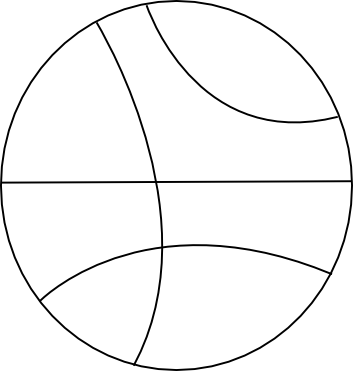
\includegraphics[width=0.5\textwidth]{PoincareDisc.png}
	\caption[A visualisation of the two dimensional Poincar\'{e} disc model containing four geodesics]{A visualisation of the two dimensional Poincar\'{e} disc model containing four geodesics \protect{\cite{poincare_model_web_page}}.}
	\label{fig:poincare_example}
\end{figure}

An example of this is shown in figure \ref{fig:poincare_example}. Here, four separate geodesics have been drawn on a hyperbolic plane and then visualised in Euclidean space using the disc model. Though these lines do not appear straight in Euclidean space the negative curvature of the hyperbolic space causes their apparent curvature in this model. Measuring an angle in this model yields the actual hyperbolic angle thus making the model conformal. Angles are determined by simply measuring the angle between the tangents of the Euclidean representation of the curves at the point they intersect.

Calculating Hyperbolic distance in the disc model is more complex than simply measuring distances in the Euclidean representation. Hyperbolic distance in the disc model, between the Euclidean points A and B, is defined as \cite{blair_inversion_2000}:

\begin{equation}
\label{distance_disc_model}
\ln(AB,PQ)
\end{equation}

where P and Q are the ideal points of the geodesic that bisects A and B. These points must be in the order P, B, A, Q on the line. (AB, PQ) is the \textit{cross-ratio} of the four points and is defined as \cite{blair_inversion_2000}:

\begin{equation}
(AB,PQ) = \frac{|AP|\cdot|BQ|}{|BP|\cdot|AQ|}
\end{equation}

where |PQ|, for example, is the Euclidean arc length between the points P and Q on the Euclidean representation of the Hyperbolic line which intersects A and B.

The further an object is from the centre of the space the more compressed it's Euclidean representation becomes, making it appear smaller. Objects near the centre of the space are represented more accurately as the compression of the Hyperbolic space is low there.

\subsection{The Beltrami-Klein Model}

The Beltrami-Klein model of hyperbolic geometry, known henceforth as the \textit{projective model} addresses the issue of the distortion of the straightness of lines but introduces a distortion of angle.

The projective model is again defined in two-dimensional Euclidean space as the open unit disc, given earlier in equation \ref{eq:open_unit_disc_eq}. A geodesic, in the projective model is any chord of the unit disc. Indeed, for a geodesic in the disc model which has ideal points A and B it is trivial to determine the equivalent in the projective model, it is simply the chord AB. The method for calculating distance is also the same as the disc model, and is defined in equation \ref{distance_disc_model}.


Figure \ref{fig:klein_example} provides an example of the model containing three geodesics. In this diagram the two topmost lines are parallel to the bottommost line and both pass through the same point, an important property of hyperbolic space. As the Hyperbolic space is effectively bent in the visualisation, Euclidean angles in this model do not correspond to the same Hyperbolic angles and this must be accounted for if the correct modelling of angles is important, as such the model is not conformal. Of course, if it is not important for angles to be accurate in the visualisation then this model may be ideal.

In order to calculate the angle between two geodesics in the projective model... TODO

\begin{figure}
	\centering
	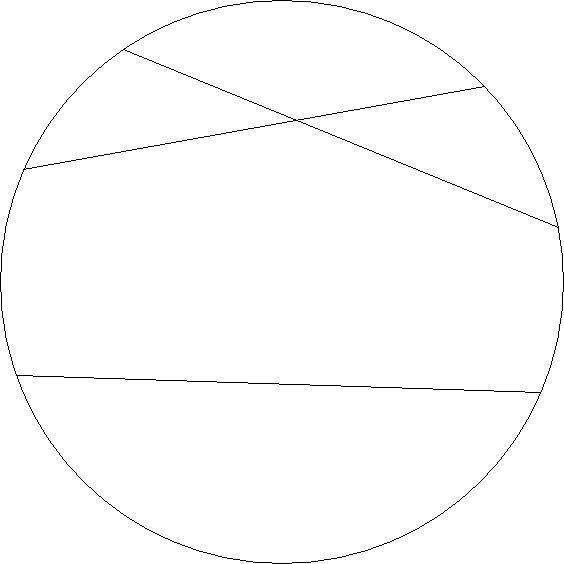
\includegraphics[width=0.5\textwidth]{Klein_model.png}
	\caption[A visualisation of the two dimensional Beltrami-Klein model containing three geodesics]{A visualisation of the two dimensional Beltrami-Klein model containing three geodesics \protect{\cite{klein_model_image}}.}
	\label{fig:klein_example}
\end{figure}

\subsection{The Poincar\'{e} Half-Plane Model}

Both models discussed previously represent the infinite hyperbolic plane inside a finite Euclidean circle, the Poincar\'{e} half-plane model, known henceforth as the \textit{half-plane} model, does not. Instead, the infinite hyperbolic space is plotted in the upper-half plane. This is a complex plane which consists of all complex numbers with a positive imaginary part. 

DEFINE UPPER HALF PLANE!!!

Figure \ref{fig:half-plane-example} shows an example of the half-plane model in which five geodesics have been plotted. In this example all of the lines on the right are parallel to the leftmost line, additionally the lines on the right also pass through a single point. The half plane model is conformal, as Euclidean angles measured in the model correspond to actual hyperbolic angles.

DISTANCES AND ANGLES!!!

\begin{figure}
	\centering
	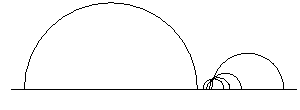
\includegraphics[width=0.75\textwidth]{upper-half-plane.png}
	\caption[A visualisation of the two dimensional Poincar\'{e} half-plane model containing five geodesics]{A visualisation of the two dimensional Poincar\'{e} half-plane model containing five geodesics \protect{\cite{half_plane_example}}.}
	\label{fig:half-plane-example}
\end{figure}

\section{Embedding Methods}
\section{Haversine Formula}